\documentclass{article}
\usepackage[utf8]{inputenc}
\usepackage{hyperref}
\usepackage{abstract}
\usepackage{geometry}
\usepackage{graphicx}
\usepackage{enumitem}
\usepackage{caption}

\renewcommand{\abstractnamefont}{\normalfont\bfseries}
\renewcommand{\abstracttextfont}{\normalfont\small\itshape}
\setlength{\absleftindent}{1cm}
\setlength{\absrightindent}{1cm}

\geometry{
  top=2cm,
  bottom=2cm,
  left=3cm,
  right=3cm
}

\hypersetup{
    colorlinks=true,
	citecolor=blue,
    linkcolor=blue,
    filecolor=magenta,      
    urlcolor=blue,
}
\usepackage[backend=biber, style=authoryear, natbib=true, url=true, doi=true, maxnames=1, minnames=1]{biblatex}
\addbibresource{references.bib}

\DeclareCiteCommand{\cite}
  {\usebibmacro{prenote}}
  {\usebibmacro{citeindex}
   \printtext[bibhyperref]{[\usebibmacro{cite}]}
  }
  {\multicitedelim}
  {\usebibmacro{postnote}}

  

\begin{document}

\title{Detection of negation and uncertainty in medical data}
\author{Amritpal Singh, Oscar Arrocha, Mustapha El Aichouni, Eric López}
\date{May 14, 2024}
\maketitle

\begin{abstract}
	In medical data analysis, accurately interpreting text, like patient information, is crucial.
	Negation and uncertainty are particularly challenging features, and misinterpreting them can
	lead to errors in medical decision-making. For this reason, this project aims to achieve a high
	precision detecting negation and uncertainty cues and their context, by developing and comparing
	two methods: a rule-based algorithm and a machine learning-based algorithm.
\end{abstract}

\section*{Rule-based method}
The goal is to build a rule-based algorithm to detect uncertainty and negation cues, and their
corresponding context, in our dataset, which consists of 318 medical documents with patient information
and a variety of medical terms. First we implement a baseline algorithm, which tags the entire sentence
after or before the negation word as its context. Then we present an implementation of NegEx \cite{negex},
which uses a simple heuristic rule to determine a more accurate context.

\subsection*{Baseline algorithm (Blind)}
Our first approach is to create a baseline model with no information about the words. That is, after
finding a negation/uncertainty word, the model will tag as scope what is behind or before the negation
(depending on its tag) until reaching at the end/start of the sentence. We call this method “blind”
because it does not take into account (it doesn’t “see”) words, only the delimiters of the sentence.
Despite this approach appearing too simplistic, it’s expected to work mostly well for most of the cases,
as many sentences have been observed to consist only of the negation and the scope, like “no hábitos tóxicos.”.

\subsubsection*{Implementation}
First, a negation list is created, where all the negations of the training set are grouped and given a tag,
based on where the position of its scope is usually found on the text (behind or after):

\begin{itemize}
	\item The tag [PREN] means that the negation is before the scope and the scope has to be tagged as [NSCO]
	\item The tag [PREP] means that the negation is before the scope and the scope has to be tagged as [USCO]
	\item The tag [POST] means that the negation is after the scope and the scope has to be tagged as [NSCO]
	\item The tag [POSP] means that the negation is before the scope and the scope has to be tagged as [USCO]
\end{itemize}

Then, this information is used to create the algorithm. First, for a given sentence, all the negations that
are spotted. Then, for each negation everything that is before/after the negation is tagged as the corresponding
scope. A weak point of this implementation is that for sentences with more than one negation, the scopes will be
overlapped.

\subsubsection*{Results}
Evaluating this algorithm in the test set yields a precision of 0.82. Recall and F1 score result in the exact
same value. As expected, the model performance at detecting the scope is reasonably high for its such simple
approach. This is because the evaluation algorithm is considering the whole text when comparing the ground
truth with the prediction, and detected negation cues and scopes are only a small part of it. This must be
taken into account for future methods explained in this report, we are aiming to achieve a high precision
relative to this one.

\subsection*{NegEx}
Once implemented a baseline model, we proceed to implement the NegEx algorithm as explained in the original
paper \cite{negex}. NegEx proposes a simple strategy to detect negation words and their scopes in medical documents:
\begin{itemize}
	\item First, the negation and uncertainty words are spotted in the sentence. 
	\item Second, the medical terms are identified in the sentence. A predefined vocabulary \footnote{The original
	paper used a union of terms from the UMLS and from ICD10. As we don’t have access to such private databases,
	our workaround consists of creating a vocabulary of medical terms by extracting all words from the scopes in the
	training set, listing them and removing those words with 3 characters or less. This is an heuristic to remove common
	determinants and conjunctions that may appear in the scopes, leaving only the medical terms, which are usually
	longer.} of these terms is necessary for this step.
	\item Finally, the negation scope is defined as the next words after the negation word until the medical term,
	included. The number of tokens that can appear in between is limited to 5. Moreover, depending on the negation
	or uncertainty word, the scope will be before or after.
\end{itemize}

\subsubsection*{Implementation}
Before implementing the NegEx algorithm, we found it beneficial to first preprocess the data. Each document is split
into sentences, and then tokenized into words. For this last step, the tokenizer works better if the language is provided,
so a first language detection step is performed over each sentence, distinguishing Catalan from Spanish.

Next, the process consists of, for each sentence, identifying the negation or uncertainty words, then the medical terms.
These steps are done by simply matching each word in our vocabulary of the corresponding terms. Finally the scope is detected,
following the definition previously explained, using an efficient and straightforward approach: a binary mask of the sentence
is created, where medical terms are 1, the rest 0. Also for each negation and uncertainty word a mask is created where words
with a distance equal or below 5 to that word are 1, the rest 0. For each word, both masks are matched using an overlapping
criteria, where only sets of 1 that intersect or are externally connected remain in the resulting mask, which represents the
scope for that word. This ensures that the scope includes at least a medical term within a distance of 5 words maximum.
The scope is saved as spans in format [start index, end index], corresponding to the indices of the characters in the original
text. In this way, sentences for each document are processed.

\subsubsection*{Results}

\begin{figure}[!t]
	\centering
	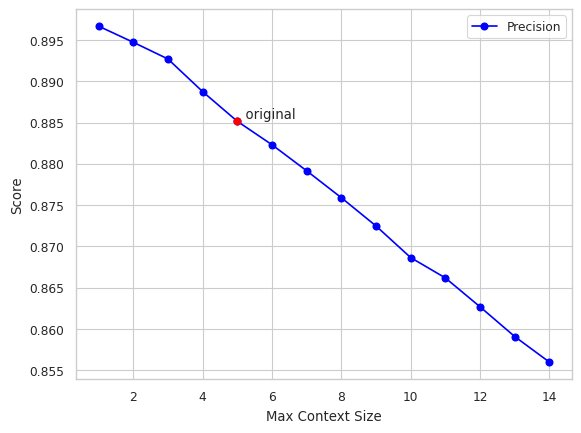
\includegraphics[height=7cm]{images/negex_context_size.jpg}
	\captionsetup{width=0.9\textwidth}
	\caption{Performance score of NegEx for different values of the maximum number of words between the negation
	or uncertainty word and the medical term. In red, the value (5) used in the original paper. Note that only
	the precision is shown, because the recall and F1 score resulted in the exact same value.}
	\label{fig:negex_context_size}
\end{figure}

By implementing NegEx as proposed in the paper, we raise all our metrics (precision, recall and F1 score) from
0.821 to 0.897 in the best case of the hyperparameter exploration, shown in Figure\ref{fig:negex_context_size}.
The best value for maximum context size is 1, in contrast to 5, used in the original paper. We believe that in
most sentences, the scope is rather close to the negation or uncertainty word, and a smaller maximum context size
reduces the chances of having overlapping scopes.

The efficiency of this algorithm is reflected in the time taken to process the documents: an average of 3.1 seconds
to process the test set, 0.05 each document. The simplicity and lower precision of this method, compared to the
next ones, is compensated with the high speed and efficiency of its implementation.

Note that in these type of natural language problems, the closer we get to a perfect accuracy, the harder it becomes
to increase the performance of the model.

\section*{Machine learning method}
Machine learning (ML) significantly enhances healthcare technology by interpreting complex data sets and training
algorithms to recognize patterns with minimal human intervention. This project applies ML to improve the processing
of medical data, specifically for detecting negation and uncertainty in patient records. 

This section details the use of ML models, algorithm selection, data preprocessing, and performance metrics. By
automating the detection process and reducing misinterpretation risks, this approach will support doctors in
delivering precise medical care and enhance the quality and reliability of medical documentation, ultimately
improving patient outcomes.

\subsection*{Conditional Random Field}
In this study, a Conditional Random Field (CRF)-based approach is employed to enhance the detection of linguistic
nuances such as negation and uncertainty within text data. The problem is treated as a Named Entity Recognition
(NER) challenge, focusing on the identification and classification of words related to negation and uncertainty.
Specifically, a tagging scheme is designed based on the BIO format to classify words under negation and uncertainty
categories:

\begin{itemize}[itemsep=0.02cm]
	\item B-NEG: Indicates beginning word of negation cue.
	\item I-NEG: Indicates inside word of negation cue.
	\item B-NSCO: Indicates beginning word of negation scope.
	\item I-NSCO: Indicates inside word of negation scope.
	\item B-UNC: Indicates beginning word of uncertainty cue.
	\item I-UNC: Indicates inside word of uncertainty cue.
	\item B-USCO: Indicates beginning word of uncertainty scope.
	\item I-USCO: Indicates inside word of uncertainty scope.
	\item O: Tags all other words that do not belong to any specific category of negation or uncertainty.
\end{itemize}

Using the above tagging, we have trained two different CRF models that differ from the features used. The models
are trained to predict these tags by learning from context-dependent features within the data, including lexical,
syntactic, and positional indicators.

\subsubsection*{Features - First Approach}
This approach focuses on providing basic features about each word to the model. Here is the list:

\begin{enumerate}[itemsep=0.02cm]
	\item TOKEN: the word itself
	\item LEMMA: the base of the word
	\item POS: the information of part of speech of the word.
	\item CHUNK: the syntactical group of the word
	\item BIAS: bias term added to the feature vector
\end{enumerate}

Additionally, the features “token”, “pos” and “chunk” of the previous word and the next are also included in the
feature vector of the current word, as well as beginning and end of sequence tokens.

\begin{figure}[!t]
	\centering
	\begin{tabular}{|c|c|c|c|c|c|c|}
		\hline
		& \multicolumn{3}{|c|}{Train} & \multicolumn{3}{|c|}{Test} \\
		\hline
		Class & Precision & Recall & F1 & Precision & Recall & F1 \\
		\hline
		B-NEG & 0.96 & 0.94 & 0.95 & 0.96 & 0.93 & 0.95 \\
		\hline
		I-NEG & 0.99 & 0.78 & 0.87 & 1.00 & 0.86 & 0.92 \\
		\hline
		B-NSCO & 0.96 & 0.91 & 0.94 & 0.97 & 0.90 & 0.93 \\
		\hline
		I-NSCO & 0.91 & 0.90 & 0.90 & 0.88 & 0.88 & 0.88 \\
		\hline
		B-UNC & 0.95 & 0.78 & 0.86 & 0.95 & 0.67 & 0.70 \\
		\hline
		I-UNC & 0.96 & 0.82 & 0.88 & 0.94 & 0.69 & 0.80 \\
		\hline
		B-USCO & 0.96 & 0.78 & 0.86 & 0.87 & 0.69 & 0.81 \\
		\hline
		I-USCO & 0.89 & 0.72 & 0.80 & 0.82 & 0.74 & 0.78 \\
		\hline
	\end{tabular}
	\captionsetup{width=0.9\textwidth}
	\caption{Train and test set results, detailing the metrics computed for each of the classes.}
	\label{fig:crf_table}
\end{figure}

\subsubsection*{Results  - First Approach}
Overall, this model performs well on both the training and test sets (with better performance on the
training set, as expected), with high precision scores indicating accurate predictions for most classes
(above 0.89 in the training set and above 0.82 in test set). However, there are challenges in capturing
all instances of certain classes, as reflected in lower recall scores. The F1-scores generally demonstrate
a good balance between precision and recall, but some classes show imbalances, particularly in the test set.

\subsubsection*{Features - Second approach}
In this approach we have used a total of 16 features as described in the original paper \cite{crf}. Here
are the complete set of features used in the training:

\begin{enumerate}[itemsep=0.02cm]
	\item WORD: the words itself.
	\item POS: the information of part of speech of the word.
	\item INIT CAP: word starts with capitalization.
	\item ALPHANUM: word consists of alphanumeric characters.
	\item HAS NUM: word contains number.
	\item HAS CAP: word contains capitalized letter.
	\item HAS DASH: word contains dash.
	\item HAS US: word contains underscore.
	\item PUNCTUATION: word contains punctuation.
	\item SUFn: suffixes in the n character length ranged from two to four.
	\item PREFn: prefixes in the n character length ranged from two to four.
	\item 2GRAMBEFORE: bigram of up to 6 words before the observed word.
	\item 2GRAMAFTER: bigram of up to 1 word after the observed word.
	\item BEFOREPOS: the information of part of speech of up to 6 words before the observed word.
	\item AFTERPOS: the information of part of speech of up to 1 word after the observed word.
	\item SPECIAL: word is one of the special words in the special dictionary. The words we included as
	special words are: ”nada”, ”ni”, ”nunca”, ”ningun”, ”ninguno”, ”ninguna”, ”alguna”, ”apenas”, ”para
	nada”, and ”ni siquiera”. These words have more tendency to be part of a negation cue with multiple
	words, in which other words may appear in between.
	\item BIAS: bias term added to the feature vector.
\end{enumerate}

With this second approach, our CRF reaches higher performance, so we decide to move forward with these
features, find optimal hyperparameters and evaluate the model.

\subsubsection*{Hyperparameter tuning - Second Approach}
\begin{figure}[!t]
	\centering
	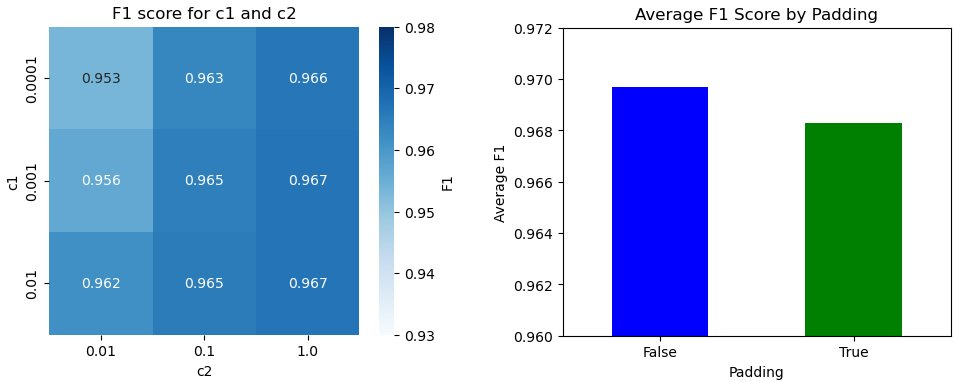
\includegraphics[height=6cm]{images/crf_heatmap_bars.jpg}
	\captionsetup{width=0.9\textwidth}
	\caption{To the left, heatmap showing the F1 score for different combinations of values for parameters
	c1 and c2. To the right, F1 score for using padding or not in context windows, an average is computed
	across different window sizes for a more stable score.}
	\label{fig:crf_heatmap_bars}
\end{figure}

Once designed the CRF and the training method, it is still possible to improve the model performance
by tuning the hyperparameters. Unlike the rule-based, with the CRF model we have  To do so, our approach
was to make a grid search to analyze the best parameter combination. The parameters our model can take
are c1 and c2 (L1 and L2 regularization, respectively), maximum number of iterations, the context window
length before and after a given token and whether to use padding. Note that a CRF can observe the information
from previous and posterior tokens. The original paper proposes those context windows to be of a maximum of 6
tokens before and 1 after.

Our grid search analysis is not exhaustive, but heuristic. The search is done in groups of parameters, so
first the optimal value is found for those parameters, and then another search is done for another group,
fixing the previous parameters to their optimal values. For this evaluation, the F1 score is used as the
performance metric, as it leverages precision and recall. Moreover these other metrics have been observed
before to be of identical value.

\begin{figure}[!t]
	\centering
	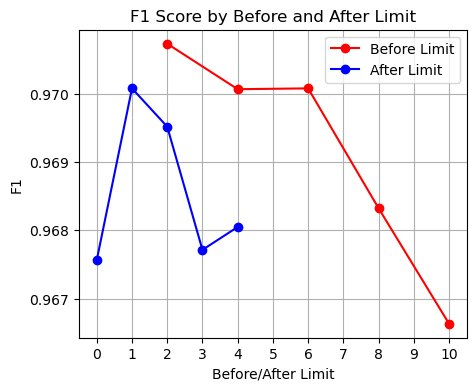
\includegraphics[height=7cm]{images/crf_lines.jpg}
	\captionsetup{width=0.9\textwidth}
	\caption{F1 score by context window length limit before and after a given token. Despite both plotted
	together, their value search has been computed separately.}
	\label{fig:crf_lines}
\end{figure}

First, the search is performed for parameters c1 and c2. As shown in Figure \ref{fig:crf_heatmap_bars},
the optimal values are a
low c1 (0.001) and a high c2 (1.0). These values are then fixed. Next, the optimal choice between using
padding or not is also found doing a grid search, this time not only with padding but also for a small
range of context window lengths before and after a token. This allows us to make a more confident choice.
The average of the F1 score is computed across these lengths, and not using padding results as the best
choice. Lastly, we confirm, as shown in Figure \ref{fig:crf_lines} that the values for the context
window length limit mentioned in the original
paper, 6 before and 1 after, are the optimal \footnote{Despite the grid search showing a length limit 2
to perform slightly better for context before, we decide to stay with the value of 6 for more stable and
informed predictions in future inferences.}.

\subsubsection*{Results - Second approach}
Now the hyperparameters are the optimal. A 5-fold cross validation is performed to ensure the training
performance, which results in a F1 score of 0.973. Finally, the model is trained on the entire training
set and evaluated on the test set, achieving a F1 score of 0.971. Comparing it with the training performance,
we confirm the model had no overfitting.

\subsection*{Results comparison: CRF, both approaches}
When comparing the two methods in terms of F1 score, the second approach achieved a higher performance,
with an F1 score of 0.971, while the first one only managed an average F1 score of 0.846. Therefore, we
can conclude that the features used in the second approach are more suitable for the task of negation
detection than the ones used in the first one.

\subsection*{Results comparison: Negex and CRF second approach}

\begin{figure}[!t]
	\centering
	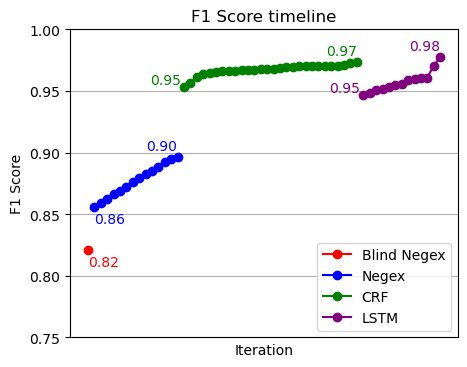
\includegraphics[height=7cm]{images/score_timeline.jpg}
	\captionsetup{width=0.9\textwidth}
	\caption{F1 scores obtained throughout this project for the different approaches, including the
	performance optimizations achieved by hyperparameter tuning. Training performance is included in
	this plot.}
	\label{fig:score_timeline}
\end{figure}

At inference time, the CRF model took 1.24 seconds to process the test set, half the time that NegEx took.
However, we must consider that the CRF required a first training step which lasted over a minute, and additional
data preprocessing (BIO labels precomputation for training set and POS tags for both sets).

Despite CRF needing extra treatment, we show in Figure \ref{fig:score_timeline} how the performance on the
task of identifying negation cues and their context is significantly increased, almost to perfection.

\section*{Conclusions}
In this study, we have implemented a Conditional Random Field (CRF)-based methodology to address the challenge
of detecting negation and uncertainty in medical texts. Our approach treats the problem as a Named Entity
Recognition (NER) task, where each word in the text is assigned a tag that indicates its role in expressing
negation or uncertainty. The CRF model predicts one of these tags for each word in a sequence, leveraging
comprehensive lexical, syntactic, and positional features for effective training.

Comparatively, the CRF model shows superior performance to the NegEx algorithm, demonstrating higher precision
and recall in detecting nuanced linguistic elements. While the CRF model is faster in processing data once
trained, it does require an initial training period which is not needed for the rule-based NegEx. Additionally,
the CRF approach necessitated more extensive data preprocessing, including the identification and incorporation
of specific lexical and syntactic features to adequately train the model. This initial investment in model
training and data preparation allows the CRF model to more accurately reflect the complexity of medical language,
thereby providing more reliable and precise analysis than the simpler NegEx method.

This comprehensive approach not only enhances the quality of medical documentation analysis but also supports
healthcare professionals by providing clearer insights into patient records, thus aiding in more accurate
clinical decision-making.


\printbibliography

\end{document}
